\section{задание: Перевод и локализация с сохранением технической специфики}
\subsection{исходные данные}
\indent Исходный текст (фрагмент): \textbf{"Para mantener la velocidad del equipo de desarrollo, es fundamental cumplir con los tiempos establecidos en la planificación. El deadline para el sprint actual es mañana al mediodía, y todavía hay tareas pendientes críticas. Por favor, revisen el backlog y actualicen el estado de sus tickets lo antes posible. No podemos cerrar el ciclo si las historias de usuario no están completas y probadas. Si hay algún bloqueo técnico, levántenlo en la reunión diaria para resolverlo antes del cierre."} \\
\indent Направление: \textbf{Spa -> Rus} \\
\indent Запрет перевода: \textbf{Agile термины (deadline, sprint, backlog)} \\
\newline
\subsection{базовый промпт}
\begin{verbatim}
					Переведи в направлении {НАПРАВЛЕНИЕ} этот текст: {ТЕКТС}
\end{verbatim}
простой запрос для перевода текста без уточнений.
\newpage
\subsection{журнал промпт-инжиниринга}
\noindent Промпт v1:
\begin{verbatim}
					Переведи в направлении Spa -> Rus этот текст: ...
\end{verbatim}
\noindent Результат (YandexGPT):
\begin{figure}[H]
	\centering
	
\includegraphics[width=17cm]{z3/a1.png}
\end{figure}
\noindent Анализ ошибок: модель полностью перевела текст даже с терминами, но выделила термины жирным. \\
Корректировка: добавить уточнение о запрете перевода терминов. \\
\newpage
\noindent Промпт v2:
\begin{verbatim}
					Переведи в направлении Spa -> Rus, но не переведи
					Agile термины (deadline, sprint, backlog). текст: ...
\end{verbatim}
\noindent Результат (YandexGPT):
\begin{figure}[H]
	\centering
	
\includegraphics[width=17cm]{z3/b1.png}
\end{figure}
\noindent Анализ ошибок: модель перевела текст, не переводя термины. \\
Корректировка: не требуется. \\
\newpage
\noindent Результат (DeepSeek):
\begin{figure}[H]
	\centering
	
\includegraphics[width=17cm]{z3/c1.png}
\end{figure}
\noindent Анализ ошибок: эта модель перевела текст аналогично. \\
Корректировка: не требуется. \\
\newpage
\noindent Результат (DeepSeek, на варианте 11):
\begin{figure}[H]
	\centering
	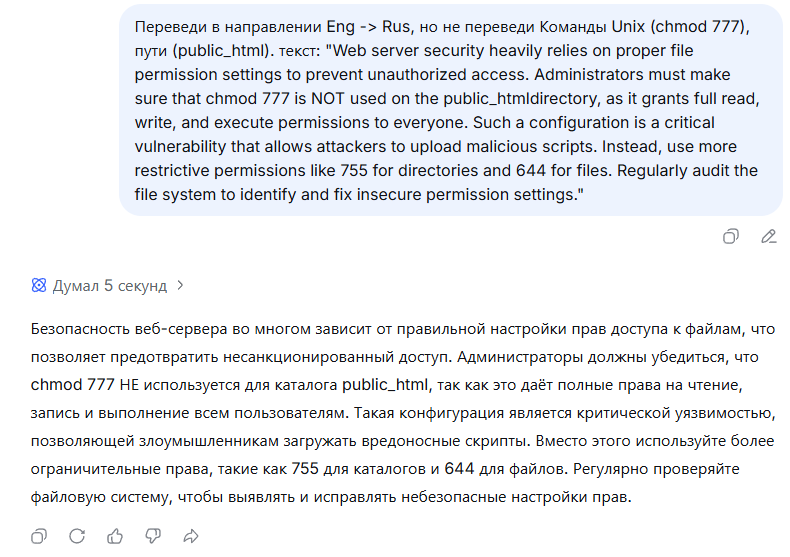
\includegraphics[width=17cm]{z3/d1.png}
\end{figure}
\noindent Анализ ошибок: данный промпт хорошо работает и для других вариантов. \\
Корректировка: не требуется. \\
\newpage
\subsection{Сравнение моделей:}
\begin{table}[h!]
	\centering
	\begin{tabular}{|l|p{5cm}|p{5cm}|}
		\hline
		\textbf{Критерий} & \textbf{YandexGPT} & \textbf{DeepSeek} \\
		\hline
		Терминологическая целостность & 5 & 5 \\
		\hline
		Сохранение  смысла & 4 & 5 \\
		\hline
		\textbf{Итог} & 4.5 & 5 \\
		\hline
	\end{tabular}
\end{table}
Модель DeepSeek справилась лучше, так как больше вникает в контекст и имеет функцию "размышления" что позволяет более точно перевести текст, зато YandexGPT быстрее обрабатывет запросы но имеет жёсткий лимит на кол-во токенов вывода.
\subsection{Финальный промпт:}
\begin{verbatim}
					Переведи в направлении {НАПРАВЛЕНИЕ}, но не переводи
					{ЗАПРЕТ_ПЕРЕВОДА}. текст: ТЕКСТ}
\end{verbatim}
\subsection{Вывод по заданию:}
\indent В данном задании лучше всего подходит техника <<Цепочка рассуждений>> так как модель лучше вникает в контекст. \\